\section{Warm up: Margins}
\label{sec:q1}

\begin{enumerate}

\item ~[5 points] Suppose we want to use an SVM to learn the XOR
  function in two dimensions. We know that XOR is not linearly
  separable, so we apply a feature transformation. In order to do so,
  we map the input $[x_1, x_2] $ into a space consisting of two
  features: $x_1$ and $x_1 x_2$. All examples are Boolean (1 for
  positive and -1 for negative) What is the maximal margin? Draw the
  separating line back in original Euclidean input space.

  \begin{table}[H]
    \centering
    \begin{tabular}{| c | c | c  |  c | }
      \hline
      $x_1$ & $x_2$  & $x_1x_2$ & $Label$ \\
      \hline
      $-1$ & $-1$ & $+1$ & $-1$\\
      $-1$ & $+1$ & $-1$ & $+1$\\
      $+1$ & $-1$ & $-1$ & $+1$\\
      $+1$ & $+1$ & $+1$ & $-1$\\
      \hline
    \end{tabular}
    \caption*{XOR Function truth table}
  \end{table}

The XOR function truth table shows the original inputs $x_1$ and $x_2$ along with the new feature $x1x2$. The label column shows $x_1 \oplus x_2$. Figure \ref{XorSvm} shows the new space with features $x_1$ and $x_1x_2$. The points in this input space are shown along with their labels. The axis for the feature $x_1$ is the linear separator with the maximum margin and is shown as the bold line. The four features in the new space become support vectors and the margin is half the distance between the lines joining the support vectors.

The input features $x_1$ and $x_2$ in the original feature space are shown in figure \ref{XorOriginal}. The lines joining the support vectors now intersect each other. The line of maximum margin in figure \ref{XorSvm} was the one where $x_1$ varied from $+\infty$ to $+\infty$ and $x_1x_2$ was $0$. The corresponding line in the original feature space would be the one where $x_1$ varies from $+\infty$ to $+\infty$ and $x_2$ is $0$, as $x_2=0$ corresponds to the case where $x_1x_2=0$ in the new feature space. This line of maximum separation is shown in bold in figure \ref{XorOriginal}.
  \begin{figure}[H]
    \centering
    \begin{tikzpicture}[domain=0:2]
      \draw[<->] (-3.2,0) -- (3.2,0) node[below right] {$x_1$};
      \draw[<->] (0,-4) -- (0,4) node[left] {$x_1x_2$};
      \draw [<->] (-3.2,3) -- (3.2,3) ;
      \draw [<->] (-3.2,-3) -- (3.2,-3) ;
      \draw [ultra thick] (-3.2,0) -- (3.2,0) ;
      \foreach \Point/\PointLabel in {(-3,3)/, (-3,-3)/, (3,-3)/, (3,3)/}
\draw[fill=black] \Point circle (0.05) node[above right] {$\PointLabel$};
\node [above] at (-3,  3) {$(-1, +1)$};
\node [below] at (-3,  3) {$ -1$};
\node [above] at (-3,  -3) {$(-1, -1)$};
\node [below] at (-3,  -3) {$ +1$};
\node [above] at (3,  -3) {$(+1, -1)$};
\node [below] at (3,  -3) {$ +1$};
\node [above] at (3,  3) {$(+1, +1)$};
\node [below] at (3,  3) {$ -1$};
    \end{tikzpicture}
    \caption{Separation of XOR function in feature space $x_1$ and $x_1x_2$.} \label{XorSvm}
  \end{figure}

  \begin{figure}[H]
    \centering
    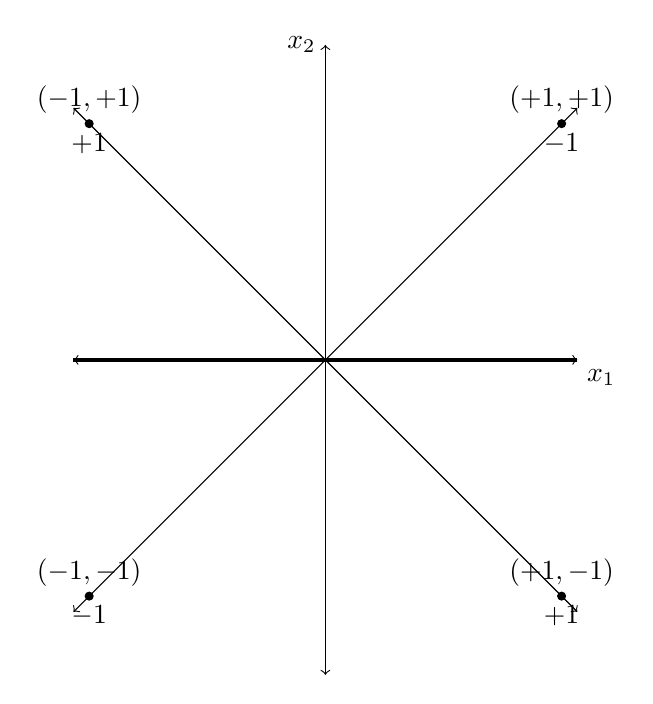
\begin{tikzpicture}[domain=0:2]
      \draw[<->] (-3.2,0) -- (3.2,0) node[below right] {$x_1$};
      \draw[<->] (0,-4) -- (0,4) node[left] {$x_2$};
      \draw [<->] (-3.2,-3.2) -- (3.2,3.2) ;
      \draw [<->] (-3.2,3.2) -- (3.2,-3.2) ;
      \draw [ultra thick] (-3.2,0) -- (3.2,0) ;
      \foreach \Point/\PointLabel in {(-3,3)/, (-3,-3)/, (3,-3)/, (3,3)/}
\draw[fill=black] \Point circle (0.05) node[above right] {$\PointLabel$};
\node [above] at (-3,  3) {$(-1, +1)$};
\node [below] at (-3,  3) {$ +1$};
\node [above] at (-3,  -3) {$(-1, -1)$};
\node [below] at (-3,  -3) {$ -1$};
\node [above] at (3,  -3) {$(+1, -1)$};
\node [below] at (3,  -3) {$ +1$};
\node [above] at (3,  3) {$(+1, +1)$};
\node [below] at (3,  3) {$ -1$};
    \end{tikzpicture}
    \caption{Separation of XOR function in original feature space $x_1$ and $x_2$.} \label{XorOriginal}
  \end{figure}
  
\item ~[10 points]  Consider the following collection of points:
  \begin{table}[H]
    \centering
    \begin{tabular}{| c | c | c  ||  c | c | c |}
      \hline
      Point & coordinate  & label & Point & coordinate  & label \\
      \hline
      $x_1$ & (0, 0)             & + & $x_5$ & (0, 1)                                & - \\
      $x_2$ & (1, 0)             & + & $x_6$ & ($\frac{1}{2}$, $\frac{\sqrt{3}}{2}$) & - \\
      $x_3$ & (1, 1)             & + & $x_7$ & ($\frac{3}{2}$, 0)                    & - \\
      $x_4$ & ($\frac{1}{2}$, 0) & + & $x_8$ & (1, $\frac{1}{2}$)                    & - \\
      \hline
    \end{tabular}
    \caption{A collection of points}
  \end{table}

  Suppose we have three training sets comprising of subsets of these
  points. We have
  $$D_1 = \{x_1, x_2, x_3, x_4, x_7\}$$
  $$D_2 = \{x_1, x_5, x_6, x_8\}$$
  $$D_3 = \{x_3, x_4, x_5, x_ 7\}$$

  \begin{enumerate}
  \item ~[6 points] Give the maximum possible margin for $D_1$, $D_2$
    and $D_3$.
   
   \begin{figure}[H]
    \centering
    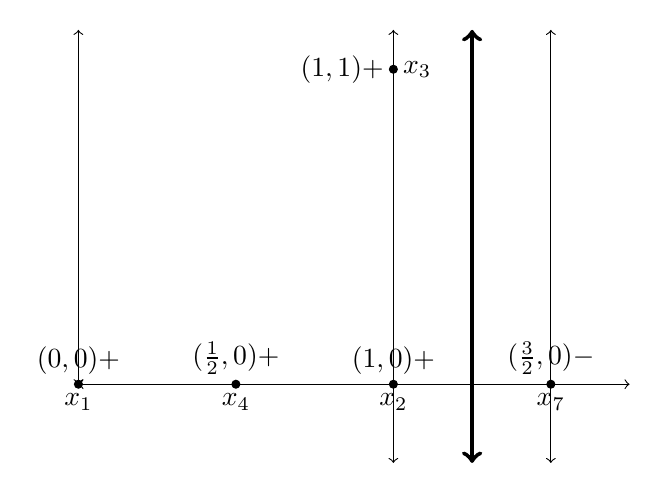
\begin{tikzpicture}[domain=0:2]
      \draw[<->] (0,0) -- (7,0);
      \draw[<->] (0,0) -- (0,4.5);
      \draw [<->] (4,-1) -- (4,4.5) ;
      \draw [<->] (6,-1) -- (6,4.5) ;
      \draw [<->] [ultra thick](5,-1) -- (5,4.5) ;
      \foreach \Point/\PointLabel in {(0,0)/, (4,0)/, (4,4)/, (2,0)/, (6,0)/}
\draw[fill=black] \Point circle (0.05) node[above right] {$\PointLabel$};
\node [above] at (0,0) {$(0,0)+$};
\node [below] at (0,0) {$x_1$};
\node [above] at (4, 0) {$(1, 0)+$};
\node [below] at (4, 0) {$x_2$};
\node [left] at (4, 4) {$(1, 1)+$};
\node [right] at (4, 4) {$x_3$};
\node [above] at (2, 0) {$(\frac{1}{2}, 0)+$};
\node [below] at (2, 0) {$x_4$};
\node [above] at (6, 0) {$(\frac{3}{2}, 0)-$};
\node [below] at (6, 0) {$x_7$};
    \end{tikzpicture}
    \caption{Points in set $D_1$.} \label{SetD1}
  \end{figure}   

The maximum margin for $D_1$ is given is shown by the solid line in figure \ref{SetD1}. This bold line is in the middle of the widest strip separating the positive and negative labels. This widest strip is shown by the two lines through $x_2$, $x_3$ and through $x_7$. The margin is thus the distance between $x_2$ and $x_7$, which is $\frac{3}{2} -1 = \frac{1}{2} =0.5$.

   
   \begin{figure}[H]
    \centering
    \begin{tikzpicture}[domain=0:2]
      \draw[<->] (-1,0) -- (10,0);
      \draw[<->] (0,-5) -- (0,4.5);
      \draw [<->] (-0.5,4.25) -- (9,-0.5) ;
      \draw [<->] (-0.5,0.25) -- (9,-4.5) ;
      \draw[] (0,0) -- (1.6,3.2);
      \draw [<->] [ultra thick](-0.5,2.25) -- (9,-2.5) ;
      \foreach \Point/\PointLabel in {(0,0)/, (0,4)/, (2,3.4641)/, (4,2)/}
\draw[fill=black] \Point circle (0.05) node[above right] {$\PointLabel$};
\node [left] at (0,0) {$(0,0)+$};
\node [below] at (0,0) {$x_1$};
\node [left] at (0, 4) {$(0, 1)-$};
\node [right] at (0, 4) {$x_5$};
\node [above] at (2, 3.4641) {$(\frac{1}{2}, \frac{\sqrt{3}}{2})-$};
\node [below] at (2, 3.4641) {$x_6$};
\node [above] at (4, 2) {$(1, \frac{1}{2})-$};
\node [below] at (4, 2) {$x_8$};
    \end{tikzpicture}
    \caption{Points in set $D_2$.} \label{SetD2}
  \end{figure}  

The widest strip separating the two labels in $D_2$ is shown in figure \ref{SetD2}, with the solid line marking the separating margin between the two labels. One side of the widest strip passes through $x_5$ and $x_8$. The slope of this line is $-\frac{1}{2}$ (computed using the formula $\frac{y_2 - y_1}{x_2 - x_1}$ for a line that passes through points $(x_1, y_1)$ and $(x_2, y_2)$). The equation of this line is $y-1=-\frac{1}{2}x$ or $x+2y=2$ (using the formula for the equation of a line that passes trough point $(x_1, y_1)$ and has a slope of $m$, which is $y-y_1 = m(x-x_1)$). The other side of the widest strip will pass through $x_1$ and will have the same slope of $-\frac{1}{2}$. So the equation of this side of the widest strip will be $x+2y=0$. The equation for the bold line separating the points with the two labels will be $x+2y=1$.

To find the width of the widest strip, we can first find the equation of the line that is perpendicular to the widest strip (slope = $2$) and passing through $(0,0)$. The equation will be $y=2x$ or $2x-y=0$. This line is shown in figure \ref{SetD2}. One end of the line is $(0,0)$ and the other end is $(0.4,0.8)$. The margin is therefore the length of this line or $\sqrt{0.4^2 + 0.8^2} = \sqrt{0.8}=0.8944$.
   
   \begin{figure}[H]
    \centering
    \begin{tikzpicture}[domain=0:2]
      \draw[<->] (0,0) -- (7,0);
      \draw[<->] (0,0) -- (0,4.5);
      \foreach \Point/\PointLabel in {(4,4)/, (2,0)/, (0,4)/,(6,0)/}
\draw[fill=black] \Point circle (0.05) node[above right] {$\PointLabel$};
\node [left] at (4, 4) {$(1, 1)+$};
\node [right] at (4, 4) {$x_3$};
\node [above] at (2, 0) {$(\frac{1}{2}, 0)+$};
\node [below] at (2, 0) {$x_4$};
\node [left] at (0, 4) {$(0, 1)-$};
\node [right] at (0, 4) {$x_5$};
\node [above] at (6, 0) {$(\frac{3}{2}, 0)-$};
\node [below] at (6, 0) {$x_7$};
    \end{tikzpicture}
    \caption{Points in set $D_3$.} \label{SetD3}
  \end{figure}   

As can be seen in figure \ref{SetD3}, the points are not linearly separable. So there os no separating margin.

  \item ~[2 points] What is the Perceptron mistake bound for these
    dataset. Which has the greatest Perceptron mistake bound.
  \item ~[2 points] Rank the datasets in terms of ``ease of
    learning''. Justify your answer.
  \end{enumerate}

\end{enumerate}


%%% Local Variables:
%%% mode: latex
%%% TeX-master: "hw"
%%% End:
